\DocumentMetadata{%
 %  uncompress, %only for debugging!!
  pdfversion=2.0,
  testphase={phase-II, tabular, graphic}%
 % testphase={phase-II,math, tabular, graphic}% TOC Does not work
   % testphase={phase-III,math}% TOC works
}
\tagpdfsetup{activate, tabsorder=structure}
% Use the following to fix bug in November 2023 download of LaTeX
\ExplSyntaxOn
\cs_generate_variant:Nn\__tag_prop_gput:Nnn{cnx}
\ExplSyntaxOff
\documentclass[11pt,
  english,
  letterpaper,
]{article}
\usepackage{sa4ss}
\usepackage{amsmath,amssymb,array}
\usepackage{booktabs}

% From tagged-template.latex
\usepackage{lmodern}
\usepackage{ifxetex,ifluatex}
\ifnum 0\ifxetex 1\fi\ifluatex 1\fi=0 % if pdftex
  \usepackage[T1]{fontenc}
  \usepackage[utf8]{inputenc}
  \usepackage{textcomp} % provide euro and other symbols
\else % if luatex or xetex
  \usepackage{unicode-math}
  \defaultfontfeatures{Scale=MatchLowercase}
  \defaultfontfeatures[\rmfamily]{Ligatures=TeX,Scale=1}
\fi

% Use upquote if available, for straight quotes in verbatim environments
\IfFileExists{upquote.sty}{\usepackage{upquote}}{}
\IfFileExists{microtype.sty}{% use microtype if available
  \usepackage[]{microtype}
  \UseMicrotypeSet[protrusion]{basicmath} % disable protrusion for tt fonts
}{}
\makeatletter
\@ifundefined{KOMAClassName}{% if non-KOMA class
  \IfFileExists{parskip.sty}{%
    \usepackage{parskip}
  }{% else
    \setlength{\parindent}{0pt}
    \setlength{\parskip}{6pt plus 2pt minus 1pt}}
}{% if KOMA class
  \KOMAoptions{parskip=half}}
\makeatother
\usepackage{xcolor}
\IfFileExists{xurl.sty}{\usepackage{xurl}}{} % add URL line breaks if available
\hypersetup{
  pdflang={en},
  hidelinks,
  pdfcreator={LaTeX via pandoc}}
\urlstyle{same} % disable monospaced font for URLs
\usepackage{longtable}
% Correct order of tables after \paragraph or \subparagraph
\usepackage{etoolbox}
\makeatletter
\patchcmd\longtable{\par}{\if@noskipsec\mbox{}\fi\par}{}{}
\makeatother
% Allow footnotes in longtable head/foot
\IfFileExists{footnotehyper.sty}{\usepackage{footnotehyper}}{\usepackage{footnote}}
\makesavenoteenv{longtable}
\usepackage{graphicx}
\makeatletter
\def\maxwidth{\ifdim\Gin@nat@width>\linewidth\linewidth\else\Gin@nat@width\fi}
\def\maxheight{\ifdim\Gin@nat@height>\textheight\textheight\else\Gin@nat@height\fi}
\makeatother
% Scale images if necessary, so that they will not overflow the page
% margins by default, and it is still possible to overwrite the defaults
% using explicit options in \includegraphics[width, height, ...]{}
\setkeys{Gin}{width=\maxwidth,height=\maxheight,keepaspectratio}
% Set default figure placement to htbp
\makeatletter
\def\fps@figure{htbp}
\makeatother
\setlength{\emergencystretch}{3em} % prevent overfull lines
\providecommand{\tightlist}{%
  \setlength{\itemsep}{0pt}\setlength{\parskip}{0pt}}
\setcounter{secnumdepth}{5}
\ifxetex
  % Load polyglossia as late as possible: uses bidi with RTL langages (e.g. Hebrew, Arabic)
  \usepackage{polyglossia}
  \setmainlanguage[]{}
\else
  \usepackage[shorthands=off,main=english]{babel}
\fi

%Define cslreferences environment, required by pandoc 2.8
%https://github.com/rstudio/rmarkdown/issues/1649
\newlength{\csllabelwidth}
\setlength{\csllabelwidth}{3em}
\newlength{\cslhangindent}
\setlength{\cslhangindent}{1.5em}
% for Pandoc 2.8 to 2.10.1
\newenvironment{cslreferences}%
  {}%
  {\par}
% For Pandoc 2.11+
\newenvironment{CSLReferences}[2] % #1 hanging-ident, #2 entry spacing
 {% don't indent paragraphs
  \setlength{\parindent}{0pt}
  % turn on hanging indent if param 1 is 1
  \ifodd #1 \everypar{\setlength{\hangindent}{\cslhangindent}}\ignorespaces\fi
  % set entry spacing
  \ifnum #2 > 0
  \setlength{\parskip}{#2\baselineskip}
  \fi
 }%
 {}
\usepackage{calc}  % for \widthof, \maxof in minipage
\newcommand{\CSLBlock}[1]{#1\hfill\break}
\newcommand{\CSLLeftMargin}[1]{\parbox[t]{\csllabelwidth}{#1}}
\newcommand{\CSLRightInline}[1]{\parbox[t]{\linewidth - \csllabelwidth}{#1}\break}
\newcommand{\CSLIndent}[1]{\hspace{\cslhangindent}#1}


\providecommand{\tightlist}{%
  \setlength{\itemsep}{0pt}\setlength{\parskip}{0pt}}


\date{}
\newcommand{\trTitle}{}
\newcommand{\trYear}{2023}
\newcommand{\trMonth}{April}
\newcommand{\trAuthsLong}{truetruetrue}
\newcommand{\trAuthsBack}{Wetzel, C.R., M.H. Monk, J. Coates}
\newcommand{\trCitation}{
\begin{hangparas}{1em}{1}
\trAuthsBack{}. \trYear{}. \trTitle{}. \glsentrylong{pfmc}, Portland, Oregon. \pageref{LastPage}{}\,p.
\end{hangparas}}

\newcommand\includegraphicsifexists[2][width=\linewidth]{\IfFileExists{#2}{\includegraphics[#1]{#2}}{}}

\begin{document}

%%%%% Frontmatter %%%%%

% Footnote symbols in front matter
\renewcommand*{\thefootnote}{\fnsymbol{footnote}}

\small
\thispagestyle{empty}
\pagenumbering{roman}
\noindent
\begin{center}
\title{}
% \textnormal{\MakeTextUppercase{\trTitle{}}}
\vspace{1.5cm}
{\Large\textbf\newline{}}

\includegraphicsifexists[width=4in]{figure_title.png}
\vfill
by\\
Chantel R. Wetzel\textsuperscript{1}\\
Melissa H. Monk\textsuperscript{2}\\
Julia Coates\textsuperscript{3}\vfill
\textsuperscript{1}Northwest Fisheries Science Center, U.S. Department of Commerce, National Oceanic and Atmospheric Administration, National Marine Fisheries Service, 2725 Montlake Boulevard East, Seattle, Washington 98112\\
\textsuperscript{2}Southwest Fisheries Science Center, U.S. Department of Commerce, National Oceanic and Atmospheric Administration, National Marine Fisheries Service, 110 McAllister Way, Santa Cruz, California 95060\\
\textsuperscript{3}.na.character\vfill
\trMonth{} \trYear{}
\end{center}
\clearpage

% Fourth page: Colophon
\thispagestyle{empty}
\vspace*{\fill}
\begin{center}
\copyright{} \glsentrylong{pfmc}, \trYear{}\\
\end{center}
\par
\bigskip
\noindent
Correct citation for this publication:
\bigskip
\par
\trCitation{}
\clearpage

% Add TOC to pdf bookmarks (clickable pdf)
\pdfbookmark[1]{\contentsname}{toc}

% Table of contents page, lists of figures and tables
\tableofcontents\clearpage
\label{TRlastRoman}
\clearpage

% Table of contents
\newpage
\thispagestyle{empty} % to remove page number

% Settings for the main document
\pagenumbering{arabic}  % Regular page numbers
\pagestyle{plain}  % No page number on first page of main document, use 'empty'
\renewcommand*{\thefootnote}{\arabic{footnote}}  % Back to numeric footnotes
\setcounter{footnote}{0}  % And start at 1
\renewcommand{\headrulewidth}{0.5pt}
\renewcommand{\footrulewidth}{0.5pt}
%\pagestyle{fancy}\fancyhead[c]{Draft: Do not cite or circulate}

\newcommand{\lt}{\ensuremath <}
\newcommand{\gt}{\ensuremath >}

\hypertarget{onboard-cpfv-index}{%
\section{Appendix C. California Onboard CPFV Index of Abundance}\label{onboard-cpfv-index}}

The state of California implemented a statewide onboard observer sampling program in 1999 (Monk et al. 2014). California Polytechnic State University (Cal Poly) has conducted an independent onboard sampling program as of 2003 for boats in Port San Luis and Morro Bay, and follows the protocols established in Reilly et al. (1998). During an onboard observer trip the sampler rides along on the CPFV and records locationspecific catch and discard information to the species level for a subset of anglers onboard the vessel. The subset of observed anglers is usually a maximum of 15 people the observed anglers change during each fishing stop.

The catch cannot be linked to an individual, but rather to a specific fishing location. The sampler also records the starting and ending time, number of anglers observed, starting and ending depth, and measures discarded fish. The fine-scale catch and effort data allow us to better filter the data for indices to fishing stops within suitable habitat for copper rockfish. Cal Poly has modified protocols reflect sampling changes that CDFW has also adopted, e.g., observing fish as they are encountered instead of at the level of a fisher's bag. Therefore, the Cal Poly data area incorporated in the same index as the CDFW data from 1999-2019. The only difference is that Cal Poly measures the length of both retained and discarded fish.

The CRFS onboard observer data went through a QA/QC process at the SWFSC which included mapping fishing drifts in ArcPro to determine if the recorded latitude and longitude were correct.

In the assessment model, the recreational CPFV fleet is modeled as retained plus discarded fish. The proportion of observed discarded copper rockfish is small, averaging 4\% over the time series (\ref{tab:onboard-keepdiscard}) and are included in the index.

We applied a number of data filters to the available data presented in Table \ref{tab:onboard-filter}. The onboard CPFV index restricts the time series to 2005-2019. The onboard observer survey began in 1999, but the sample sizes were small during the first year of the program. The years 1999-2004 also represent years where a number of regulations changed including gear limits, bag limits, and spatial closures. Due to COVID-19, no onboard sampling took place in 2020. In 2021 the onboard sampling resumed in August, at which point a large portion of the southern California fleet had switched target species and fish highly migratory species. The 2021 stock assessment had also been released by August 2021 indicating the stock was below the biomass at 40\%. The southern California CPFV began an organized effort to avoid copper rockfish and encourage their clientele to release and descend copper rockfish when encountered. In 2022, the CDFW implemented the one copper rockfish sub-bag limit and combined with avoidance by the fleet, does not represent the available copper rockfish biomass. See the online supplementary material or the history of regulation changes section for details.

The filters also included removal of the number of observed anglers and time fished at the tail ends of the distributions, remooval of drifts occurring in depths outside copper rockfish's range (Table \ref{tab:onboard-filter} and Figure \ref{fig:onboard-depths}). Because the availability of high resolution data were lacking for the south, we retained all drifts from within a CDFW block that had at least 100 drifts and at least 5\% of those encountered copper rockfish. We retained 17,605 drifts for index standardization, and 3,035 of those drifts encountered copper rockfish Table \ref{tab:onboard-percentpos}.

We modeled catch per angler minutes fished (CPUE) by fishing drift. Prior to any modeling, the SWFSC QA/QC'd the data to ensure the location information was correct. Each drift was overlaid with the available interpreted substrate layer that characterizes rocky and hard substrate, assigned to a rocky reef and the distance of the drift start location calculated. In addition, the depth of the start location was interpreted from the 2 m resolution bathymetry as well as 90 m resolution bathymetry layer for comparison. For drifts missing depth location, we assigned depth based on the best available depth based on the bathymetry.

To appropriately weight the onboard observer survey index by the available rocky substrate within a region, each drift was assigned to the closest area of rocky habitat. Hard bottom was extracted from the \href{http://seafloor.otterlabs.org/index.html}{California Seafloor Mapping Project}, along the mainland coast of southern California. These data were collected in state waters at a resolution of two meters, but did not extend into state waters past the mainland coast. Additional interpreted bathymetric data classifying the bottom type as rock or soft bottom were compiled by analysts at the University of California Santa Cruz and are now also available from CDFW's website. We used the available interepreted rocky substrate data to expand the known area of rocky substrate to areas in southern California that lack substrate type. This expansion of the estiamated rocky substrate assumes that the proportions of rocky substrate within and outside state waters are similar. Copper rockfish are a nearshore species and the majority of observed encounters were within state waters (Table \ref{tab:onboard-waterarea}). is a course estimation of the amount of rocky substrate, and represents the best available data. The calculations can be found in the online supplementary material.

The covariates explored for model selection included year and four levels region as categorical region (District 1 mainland, District 2 mainland, Southern Channel Islands and Northern Channel Islands), a year and area interaction, categorical variable for month, and continuous depth and depth-squared. rends in the average CPUE by region were similar in the filtered data set (Figure \ref{fig:onboard-regioncpue}). A year and region interaction was included after visualizing the trends in average CPUE over time (Figure @ref(fig:onboard-average\_cpue\_by\_region)). The full model was selected by AICc (Table @ref(tab:onboard-model\_selection)). In southern California, whether a trip is a 1/3 or 3/4 or overnight trip has a significant impact on the available fishing grounds. The 1/2 day CPFV vessels fishnthe shallower, nearshore waters along the along the mainland areas. The 3/4 and overnight or multi-day vessels are able to access the same areas of the Northern Channel Islands, where as the southern Channel Islands are further offshore and the observations are predominantly from overnight trips. The overnight and multi-day trips may target multiple target species, i.e., tuna and rockfish, depending on the time of the year.

Indices were fit via MLE from the sdmTMB package in R. The QQ plot fot the negative binoimal model indicated a poor fit to the data, which as not surprising given the low percent of observed drifts encountering copper rockfish. A delta-Lognormal was selected over a delta-gamma by a delta AIC of xxxxx. The QQ plot indicated a much improved fit compared to the negative binomaial model (Table \ref{fig:onboard-qq}).

The final index was weighted based on the estimates of rocky substrate within each of the four regions. The relative abundance increases during the first part of the time series (Table \ref{tab:onboard-index} and Figure \ref{fig:onboard-index}).

\begingroup\fontsize{10}{12}\selectfont
\begingroup\fontsize{10}{12}\selectfont

\begin{longtable}[t]{c>{\centering\arraybackslash}p{2cm}>{\centering\arraybackslash}p{2cm}>{\centering\arraybackslash}p{2cm}}
\caption{\label{tab:onboard-keepdiscard}Number of observed copper rockfish retained and discarded by year.}\\
\toprule
Year & Number Kept & Number Discarded & Proportion discarded\\
\midrule
\endfirsthead
\caption[]{\label{tab:onboard-keepdiscard}Number of observed copper rockfish retained and discarded by year. \textit{(continued)}}\\
\toprule
Year & Number Kept & Number Discarded & Proportion discarded\\
\midrule
\endhead

\endfoot
\bottomrule
\endlastfoot
1999 & 188 & 2 & 1.1\%\\
2000 & 87 & 1 & 1.1\%\\
2001 & 20 & 2 & 9.1\%\\
2002 & 57 & 14 & 19.7\%\\
2003 & 109 & 8 & 6.8\%\\
2004 & 142 & 6 & 4.1\%\\
2005 & 231 & 20 & 8.0\%\\
2006 & 277 & 51 & 15.5\%\\
2007 & 387 & 38 & 8.9\%\\
2008 & 388 & 21 & 5.1\%\\
2009 & 347 & 21 & 5.7\%\\
2010 & 409 & 7 & 1.7\%\\
2011 & 566 & 18 & 3.1\%\\
2012 & 865 & 69 & 7.4\%\\
2013 & 1227 & 159 & 11.5\%\\
2014 & 652 & 52 & 7.4\%\\
2015 & 716 & 40 & 5.3\%\\
2016 & 742 & 33 & 4.3\%\\
2017 & 598 & 19 & 3.1\%\\
2018 & 575 & 19 & 3.2\%\\
2019 & 449 & 17 & 3.6\%\\*
\end{longtable}
\endgroup{}
\endgroup{}

\newpage

\begingroup\fontsize{10}{12}\selectfont
\begingroup\fontsize{10}{12}\selectfont

\begin{longtable}[t]{c>{\centering\arraybackslash}p{2.2cm}>{\centering\arraybackslash}p{2.2cm}>{\centering\arraybackslash}p{2.2cm}>{\centering\arraybackslash}p{2.2cm}}
\caption{\label{tab:onboard-waterarea}Number of observed drifts inside and outside of state waters.}\\
\toprule
District & Year & Inside State Waters & Outside State Waters & Percent Inside\\
\midrule
\endfirsthead
\caption[]{\label{tab:onboard-waterarea}Number of observed drifts inside and outside of state waters. \textit{(continued)}}\\
\toprule
District & Year & Inside State Waters & Outside State Waters & Percent Inside\\
\midrule
\endhead

\endfoot
\bottomrule
\endlastfoot
1 & 2005 & 18 & 3 & 85.7\%\\
1 & 2006 & 48 & 11 & 81.4\%\\
1 & 2007 & 55 & 8 & 87.3\%\\
1 & 2008 & 43 & 14 & 75.4\%\\
1 & 2009 & 45 & 6 & 88.2\%\\
1 & 2010 & 31 & 6 & 83.8\%\\
1 & 2011 & 51 & 21 & 70.8\%\\
1 & 2012 & 63 & 15 & 80.8\%\\
1 & 2013 & 97 & 32 & 75.2\%\\
1 & 2014 & 71 & 16 & 81.6\%\\
1 & 2015 & 75 & 22 & 77.3\%\\
1 & 2016 & 86 & 43 & 66.7\%\\
1 & 2017 & 57 & 27 & 67.9\%\\
1 & 2018 & 41 & 16 & 71.9\%\\
1 & 2019 & 26 & 11 & 70.3\%\\
2 & 2005 & 31 & 6 & 83.8\%\\
2 & 2006 & 48 & 1 & 98.0\%\\
2 & 2007 & 78 & 14 & 84.8\%\\
2 & 2008 & 89 & 1 & 98.9\%\\
2 & 2009 & 51 & 0 & 100.0\%\\
2 & 2010 & 67 & 0 & 100.0\%\\
2 & 2011 & 130 & 8 & 94.2\%\\
2 & 2012 & 246 & 26 & 90.4\%\\
2 & 2013 & 302 & 14 & 95.6\%\\
2 & 2014 & 180 & 11 & 94.2\%\\
2 & 2015 & 127 & 60 & 67.9\%\\
2 & 2016 & 106 & 16 & 86.9\%\\
2 & 2017 & 111 & 8 & 93.3\%\\
2 & 2018 & 131 & 38 & 77.5\%\\
2 & 2019 & 72 & 5 & 93.5\%\\*
\end{longtable}
\endgroup{}
\endgroup{}

\newpage

\begingroup\fontsize{10}{12}\selectfont
\begingroup\fontsize{10}{12}\selectfont

\begin{longtable}[t]{c>{\centering\arraybackslash}p{2.2cm}>{\centering\arraybackslash}p{2.2cm}>{\centering\arraybackslash}p{2.2cm}>{\centering\arraybackslash}p{2.2cm}}
\caption{\label{tab:onboard-percentpos}Data filtering steps for the onboard CPFV survey.}\\
\toprule
Year & Trips with Target & Trips without Target & Total trips & Percent with Target\\
\midrule
\endfirsthead
\caption[]{\label{tab:onboard-percentpos}Data filtering steps for the onboard CPFV survey. \textit{(continued)}}\\
\toprule
Year & Trips with Target & Trips without Target & Total trips & Percent with Target\\
\midrule
\endhead

\endfoot
\bottomrule
\endlastfoot
2005 & 54 & 549 & 603 & 9.0\%\\
2006 & 95 & 708 & 803 & 11.8\%\\
2007 & 151 & 763 & 914 & 16.5\%\\
2008 & 144 & 1010 & 1154 & 12.5\%\\
2009 & 101 & 1018 & 1119 & 9.0\%\\
2010 & 104 & 957 & 1061 & 9.8\%\\
2011 & 206 & 985 & 1191 & 17.3\%\\
2012 & 335 & 1128 & 1463 & 22.9\%\\
2013 & 427 & 1227 & 1654 & 25.8\%\\
2014 & 270 & 1024 & 1294 & 20.9\%\\
2015 & 278 & 1182 & 1460 & 19.0\%\\
2016 & 245 & 1137 & 1382 & 17.7\%\\
2017 & 199 & 1160 & 1359 & 14.6\%\\
2018 & 220 & 953 & 1173 & 18.8\%\\
2019 & 110 & 865 & 975 & 11.3\%\\*
\end{longtable}
\endgroup{}
\endgroup{}

\newpage

\begingroup\fontsize{10}{12}\selectfont
\begingroup\fontsize{10}{12}\selectfont

\begin{longtable}[t]{c>{\centering\arraybackslash}p{2cm}>{\centering\arraybackslash}p{2cm}>{\centering\arraybackslash}p{2cm}}
\caption{\label{tab:onboard-filter}Data filtering steps for the onboard CPFV survey.}\\
\toprule
Filter & Description & Number of Samples & Positive Samples\\
\midrule
\endfirsthead
\caption[]{\label{tab:onboard-filter}Data filtering steps for the onboard CPFV survey. \textit{(continued)}}\\
\toprule
Filter & Description & Number of Samples & Positive Samples\\
\midrule
\endhead

\endfoot
\bottomrule
\endlastfoot
All data & All data & 56276 & 4861\\
Years & Start time series in 2005 due to sparse data & 46125 & 4523\\
Errors and Missing Data & Remove drifts with missing data and identified errors & 41837 & 4319\\
Area fished & Remove drifts in bays and Mexico (if applicable) & 39081 & 4235\\
Months fished & Remove Jan-Feb; recreational rockfish fishery closed & 35123 & 4112\\
Depth & Remove drifts in depths greater than 60 fathoms & 33724 & 4094\\
Observed anglers & Remove upper and lower 2.5\% of observed anglers; 
                                           Remaining data: Observed anglers 4-14 & 32603 & 3977\\
Time fished & Remove upper and lower 2.5\% time fished and 
                                         time fished; Remaining drifts with 5-102 minutes time fished & 29641 & 3773\\
Distance from rocky substrate & Southern CA rocky substrate incomplete; 
                                         keep 95\% of the data; drifts within 3,365 m of rocky substrate & 25099 & 3381\\
CDFW block & Retain drifts in CDFW blocks with at least 100 drifts and 
                                         more than 5\% of all drifts in that block 
                                         caught a copper rockfish & 17605 & 3035\\*
\end{longtable}
\endgroup{}
\endgroup{}

\newpage

\begingroup\fontsize{10}{12}\selectfont
\begingroup\fontsize{10}{12}\selectfont

\begin{longtable}[t]{c>{\centering\arraybackslash}p{1.22cm}>{\centering\arraybackslash}p{1.22cm}>{\centering\arraybackslash}p{1.22cm}>{\centering\arraybackslash}p{1.22cm}>{\centering\arraybackslash}p{1.22cm}>{\centering\arraybackslash}p{1.22cm}>{\centering\arraybackslash}p{1.22cm}>{\centering\arraybackslash}p{1.22cm}}
\caption{\label{tab:onboard-modelselect}Model selection for the onboard CPFV survey.}\\
\toprule
Depth & Month & Region & Year & Effort.Offset & Df & Log.Likelihood & AICc & Delta\\
\midrule
\endfirsthead
\caption[]{\label{tab:onboard-modelselect}Model selection for the onboard CPFV survey. \textit{(continued)}}\\
\toprule
Depth & Month & Region & Year & Effort.Offset & Df & Log.Likelihood & AICc & Delta\\
\midrule
\endhead

\endfoot
\bottomrule
\endlastfoot
0.035 & + & + & + & + & 35 & -13212.2 & 26494.6 & 0.0\\
0.040 & NA & + & + & + & 26 & -13368.2 & 26788.4 & 293.8\\
NA & + & + & + & + & 34 & -13418.5 & 26905.2 & 410.6\\
NA & NA & + & + & + & 25 & -13653.7 & 27357.5 & 862.9\\
0.060 & + & NA & + & + & 32 & -14764.8 & 29593.7 & 3099.1\\
0.062 & NA & NA & + & + & 23 & -14824.1 & 29694.2 & 3199.7\\
NA & + & NA & + & + & 31 & -15196.4 & 30454.9 & 3960.3\\
NA & NA & NA & + & + & 22 & -15289.1 & 30622.3 & 4127.8\\*
\end{longtable}
\endgroup{}
\endgroup{}

\newpage

\begingroup\fontsize{10}{12}\selectfont
\begingroup\fontsize{10}{12}\selectfont

\begin{longtable}[t]{c>{\centering\arraybackslash}p{2cm}>{\centering\arraybackslash}p{2cm}}
\caption{\label{tab:onboard-index}Estimated relative index of abundance for the onboard CPFV survey.}\\
\toprule
Year & Estimate & logSE\\
\midrule
\endfirsthead
\caption[]{\label{tab:onboard-index}Estimated relative index of abundance for the onboard CPFV survey. \textit{(continued)}}\\
\toprule
Year & Estimate & logSE\\
\midrule
\endhead

\endfoot
\bottomrule
\endlastfoot
2005 & 0.0061347 & 0.2172645\\
2006 & 0.0049488 & 0.1567635\\
2007 & 0.0084932 & 0.1369000\\
2008 & 0.0068229 & 0.1362750\\
2009 & 0.0040240 & 0.1715177\\
2010 & 0.0048517 & 0.1616946\\
2011 & 0.0061762 & 0.1264844\\
2012 & 0.0096174 & 0.1108631\\
2013 & 0.0126456 & 0.0904406\\
2014 & 0.0103989 & 0.1083148\\
2015 & 0.0133946 & 0.1079517\\
2016 & 0.0119204 & 0.1193485\\
2017 & 0.0097312 & 0.1223072\\
2018 & 0.0138871 & 0.1473609\\
2019 & 0.0069873 & 0.1706739\\*
\end{longtable}
\endgroup{}
\endgroup{}

\newpage

\includegraphics[width=1\textwidth,height=1\textheight]{S:/copper_rockfish_2023/data/rec_indices/crfs_cpfv_onboard/south/copper_depths_gisdepthadded.png} \newpage

\begin{figure}
\centering
\includegraphics[width=1\textwidth,height=1\textheight]{S:/copper_rockfish_2023/data/rec_indices/crfs_cpfv_onboard/south/drifts_by_depth_district.png}
\caption{Stacked bar plot of the depth of observed copper rockfish by district.\label{fig:onboard-depths}}
\end{figure}

\newpage

\begin{figure}
\centering
\includegraphics[width=1\textwidth,height=1\textheight]{S:/copper_rockfish_2023/data/rec_indices/crfs_cpfv_onboard/south/start2005/average_cpue_by_region.png}
\caption{Average CPUE by region prior to standardization.\label{fig:onboard-regioncpue}}
\end{figure}

\newpage

\begin{figure}
\centering
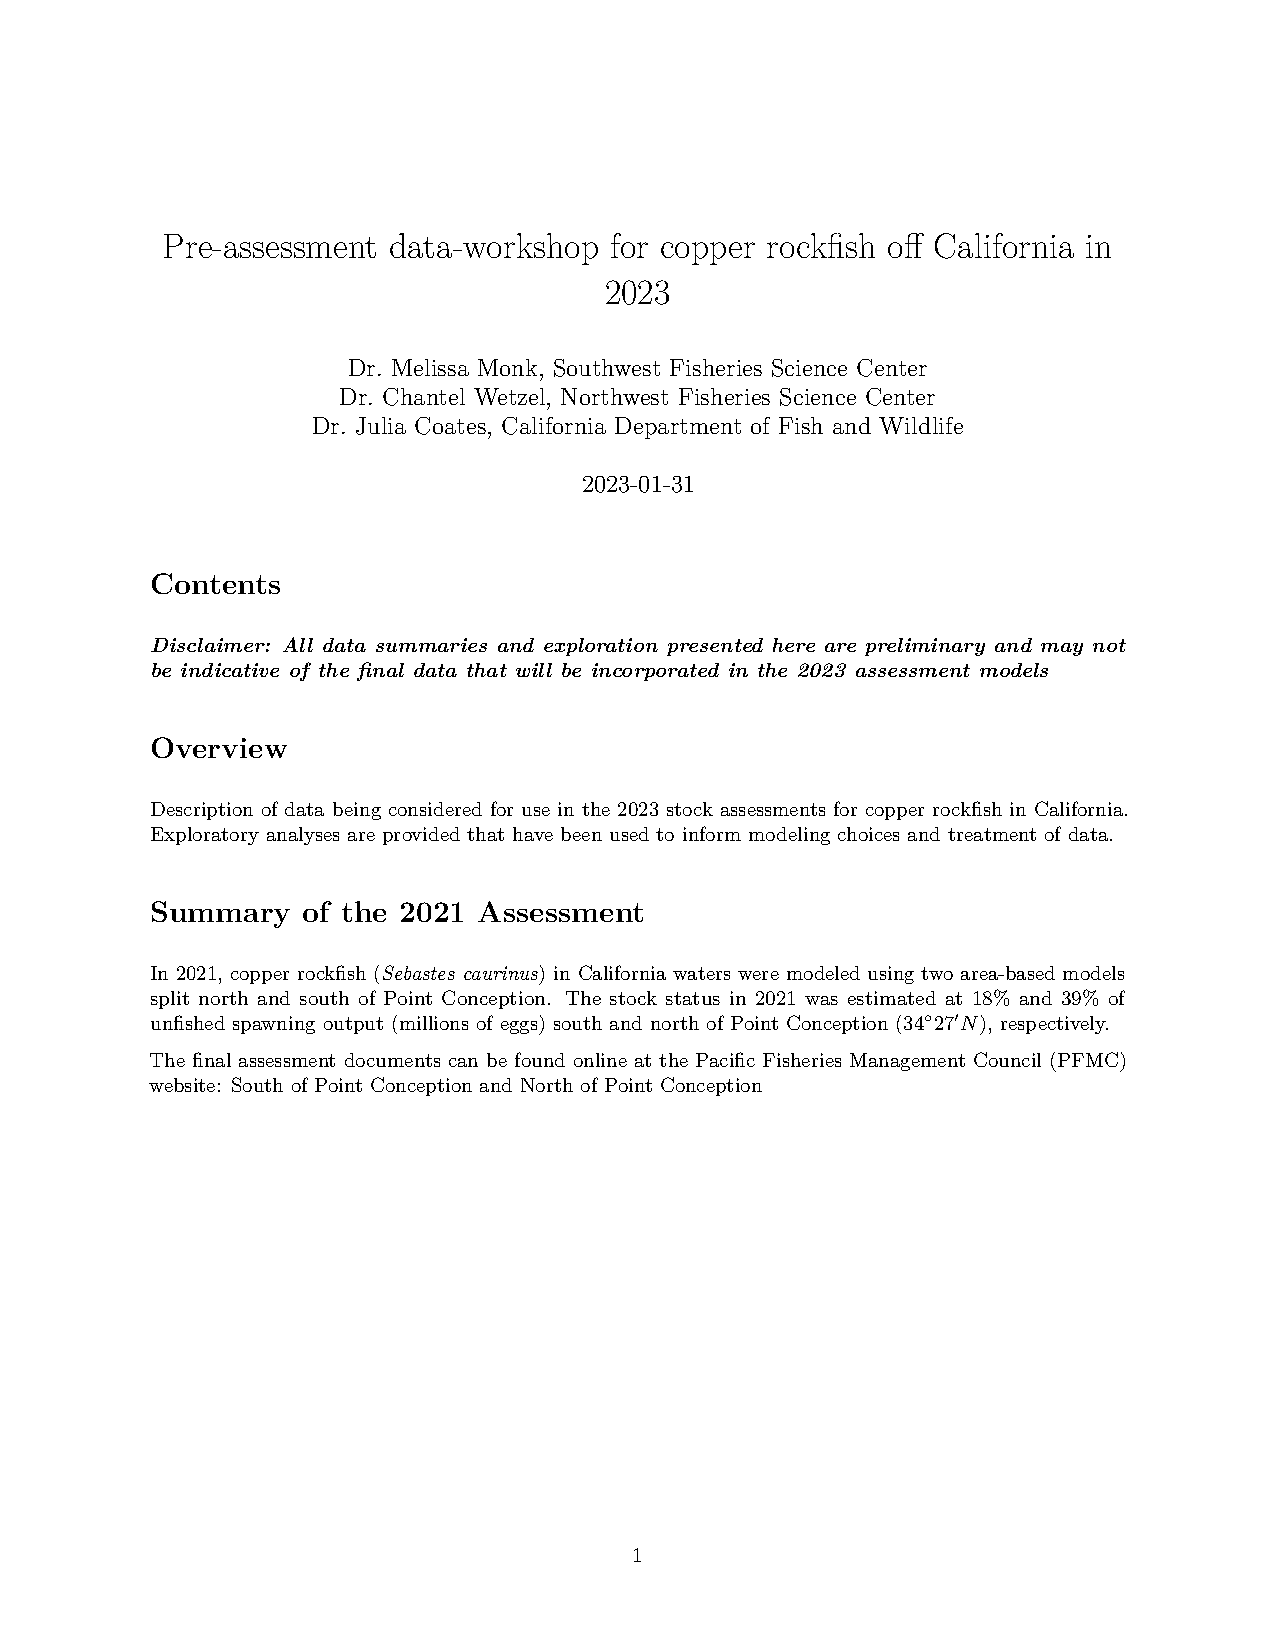
\includegraphics[width=1\textwidth,height=1\textheight]{S:/copper_rockfish_2023/data/rec_indices/crfs_cpfv_onboard/south/start2005/area_weighted_logn/index.png}
\caption{Index for the onboard CPFV survey.\label{fig:onboard-index}}
\end{figure}

\newpage

\begin{figure}
\centering
\includegraphics[width=1\textwidth,height=1\textheight]{S:/copper_rockfish_2023/data/rec_indices/crfs_cpfv_onboard/south/start2005/area_weighted_logn/qq.png}
\caption{QQ-plot for the onboard CPFV survey.\label{fig:onboard-qq}}
\end{figure}

\newpage

\hypertarget{refs}{}
\begin{CSLReferences}{1}{0}
\leavevmode\vadjust pre{\hypertarget{ref-monk_documentation_2014}{}}%
Monk, M.H., Dick, E.J., and Pearson, D. 2014. Documentation of a relational database for the {California} recreational fisheries survey onboard observer sampling program, 1999-2011. NOAA-TM-NMFS-SWFSC-529.

\leavevmode\vadjust pre{\hypertarget{ref-reilly_onboard_1998}{}}%
Reilly, P.N., Wilson-Vandenberg, D., Wilson, C.E., and Mayer, K. 1998. Onboard sampling of the rockfish and lingcod commercial passenger fishing vessel industry in northern and central {California}, {January} through {December} 1995. Marine region, Admin. Rep. \textbf{98-1}: 1--110.

\end{CSLReferences}
\end{document}
